\section{Estudio de las comunidades en la red}

De cara a realizar este estudio se han utilizado los algoritmos de Lovaina y el de Leiden. Debido a que la red cuenta con un gran número de componentes conexas, pero la mayoría se tratan de nodos aislados, se utilizará únicamente la componente gigante de la red.

\subsection{Método de Lovaina}

Se ha lanzado el método de Lovaina para distintos valores de resolución, obteniendo los siguientes resultados:

\begin{table}[H]
\centering
\begin{tabular}{|r|r|r|}
\hline
\multicolumn{1}{|c|}{\textbf{Resolución}} & \multicolumn{1}{c|}{\textbf{Modularidad}} & \multicolumn{1}{c|}{\textbf{Número de comunidades}} \\ \hline
\textit{0,25}                             & \textit{0,139}                            & \textit{89}                                         \\ \hline
\textit{0,5}                              & \textit{0,222}                            & \textit{26}                                         \\ \hline
\textit{1.0}                              & \textit{0,297}                            & \textit{5}                                          \\ \hline
\textit{1,5}                              & \textit{0,257}                            & \textit{3}                                          \\ \hline
\textit{2,5}                              & \textit{0}                                & \textit{1}                                          \\ \hline
\end{tabular}
\caption{Resultados de las ejecuciones del método de Lovaina sobre la componente gigante de la red.}
\end{table}


En este caso la ejecución que mejor ha funcionado ha sido la ejecución con resolución 1, su valor por defecto. Aun así, el valor de modularidad es bajo, apenas llegando al $0.3$, con el que se consiguen cinco comunidades. El resto de valores empeoran el resultado de modularidad, y como era de esperar, un valor más bajo de resolución hace una mayor división en comunidades, mientras que con un valor un poco más alto de modularidad apenas conseguimos dividir la red.

Este valor de modularidad tan bajo es normal en este caso, al encontrarnos con una red tan cohesionada. Vamos a pasar a analizar los resultados obtenidos para valor de resolución:


\begin{table}[H]
\centering
\resizebox{\textwidth}{!}{%
\begin{tabular}{|r|r|r|r|r|}
\hline
\multicolumn{1}{|c|}{\textbf{Número de comunidad}} & \multicolumn{1}{c|}{\textbf{Número de nodos}} & \multicolumn{1}{c|}{\textbf{Porcentaje de nodos}} & \multicolumn{1}{c|}{\textbf{Número de enlaces}} & \multicolumn{1}{c|}{\textbf{Porcentaje de enlaces}} \\ \hline
\textit{Comunidad 0}                               & \textit{18}                                   & \textit{0,97}                                     & \textit{22}                                     & \textit{0,05}                                       \\ \hline
\textit{Comunidad 1}                               & \textit{9}                                    & \textit{0,49}                                     & \textit{38}                                     & \textit{0,06}                                       \\ \hline
\textit{Comunidad 2}                               & \textit{55}                                   & \textit{2,97}                                     & \textit{501}                                    & \textit{1,06}                                       \\ \hline
\textit{Comunidad 3}                               & \textit{33}                                   & \textit{1,78}                                     & \textit{366}                                    & \textit{0,77}                                       \\ \hline
\textit{Comunidad 4}                               & \textit{12}                                   & \textit{0,65}                                     & \textit{15}                                     & \textit{0,03}                                       \\ \hline
\end{tabular}
}
\caption{Primeras cinco comunidades obtenidas para un valor de resolución de $0.25$.}
\end{table}

Como era de esperar, en este caso vemos como se han obtenido comunidades muy pequeñas, sin llegar a los 100 nodos en ninguna de ellas, por lo que se ha particionado demasiado la red y por lo tanto no podemos sacar ninguna conclusión de estos resultados. He decidido poner únicamente las cinco primeras comunidades en la tabla ya que el resto eran similares y no añadía información.


% Please add the following required packages to your document preamble:
% \usepackage{graphicx}
\begin{table}[H]
\centering
\resizebox{\textwidth}{!}{%
\begin{tabular}{|r|r|r|r|r|}
\hline
\multicolumn{1}{|c|}{\textbf{Número de comunidad}} & \multicolumn{1}{c|}{\textbf{Número de nodos}} & \multicolumn{1}{c|}{\textbf{Porcentaje de nodos}} & \multicolumn{1}{c|}{\textbf{Número de enlaces}} & \multicolumn{1}{c|}{\textbf{Porcentaje de enlaces}} \\ \hline
\textit{Comunidad 0}                               & \textit{76}                                   & \textit{4,1}                                      & \textit{613}                                    & \textit{1,3}                                        \\ \hline
\textit{Comunidad 1}                               & \textit{126}                                  & \textit{6,8}                                      & \textit{2470}                                   & \textit{5,22}                                       \\ \hline
\textit{Comunidad 2}                               & \textit{145}                                  & \textit{7,83}                                     & \textit{1464}                                   & \textit{3,09}                                       \\ \hline
\textit{Comunidad 3}                               & \textit{127}                                  & \textit{6,86}                                     & \textit{2373}                                   & \textit{5,01}                                       \\ \hline
\textit{Comunidad 4}                               & \textit{28}                                   & \textit{1,51}                                     & \textit{74}                                     & \textit{0,16}                                       \\ \hline
\end{tabular}%
}
\caption{Primeras cinco comunidades obtenidas para un valor de resolución de $0.5$.}
\end{table}

Para el caso de resolución $0.5$, ya comenzamos a ver divisiones con más nodos, sin embargo nos seguimos encontrando con comunidades muy pequeñas, sin aportar mucha información.


% Please add the following required packages to your document preamble:
% \usepackage{graphicx}
\begin{table}[H]
\centering
\resizebox{\textwidth}{!}{%
\begin{tabular}{|r|r|r|r|r|}
\hline
\multicolumn{1}{|c|}{\textbf{Número de comunidad}} & \multicolumn{1}{c|}{\textbf{Número de nodos}} & \multicolumn{1}{c|}{\textbf{Porcentaje de nodos}} & \multicolumn{1}{c|}{\textbf{Número de enlaces}} & \multicolumn{1}{c|}{\textbf{Porcentaje de enlaces}} \\ \hline
\textit{Comunidad 0}                               & \textit{339}                                  & \textit{18,3}                                     & \textit{2074}                                   & \textit{4,38}                                       \\ \hline
\textit{Comunidad 1}                               & \textit{513}                                  & \textit{27,7}                                     & \textit{7572}                                   & \textit{16}                                         \\ \hline
\textit{Comunidad 2}                               & \textit{232}                                  & \textit{12,53}                                    & \textit{4492}                                   & \textit{9,49}                                       \\ \hline
\textit{Comunidad 3}                               & \textit{321}                                  & \textit{17,33}                                    & \textit{7992}                                   & \textit{16,88}                                      \\ \hline
\textit{Comunidad 4}                               & \textit{447}                                  & \textit{24,14}                                    & \textit{3557}                                   & \textit{7,51}                                       \\ \hline
\end{tabular}%
}
\caption{Cinco comunidades obtenidas para un valor de resolución de $1$.}
\end{table}

El caso de resolución $1$ es el caso donde se ha obtenido mejor modularidad, y donde podemos observar que tienen más sentido las comunidades escogidas, por lo que en este punto voy a realizar un análisis más exhaustivo.



Para comenzar, vamos a visualizar la red completa, así como las diferentes comunidades obtenidas por separado:



\newpage
\begin{figure}[H]
	\centering
	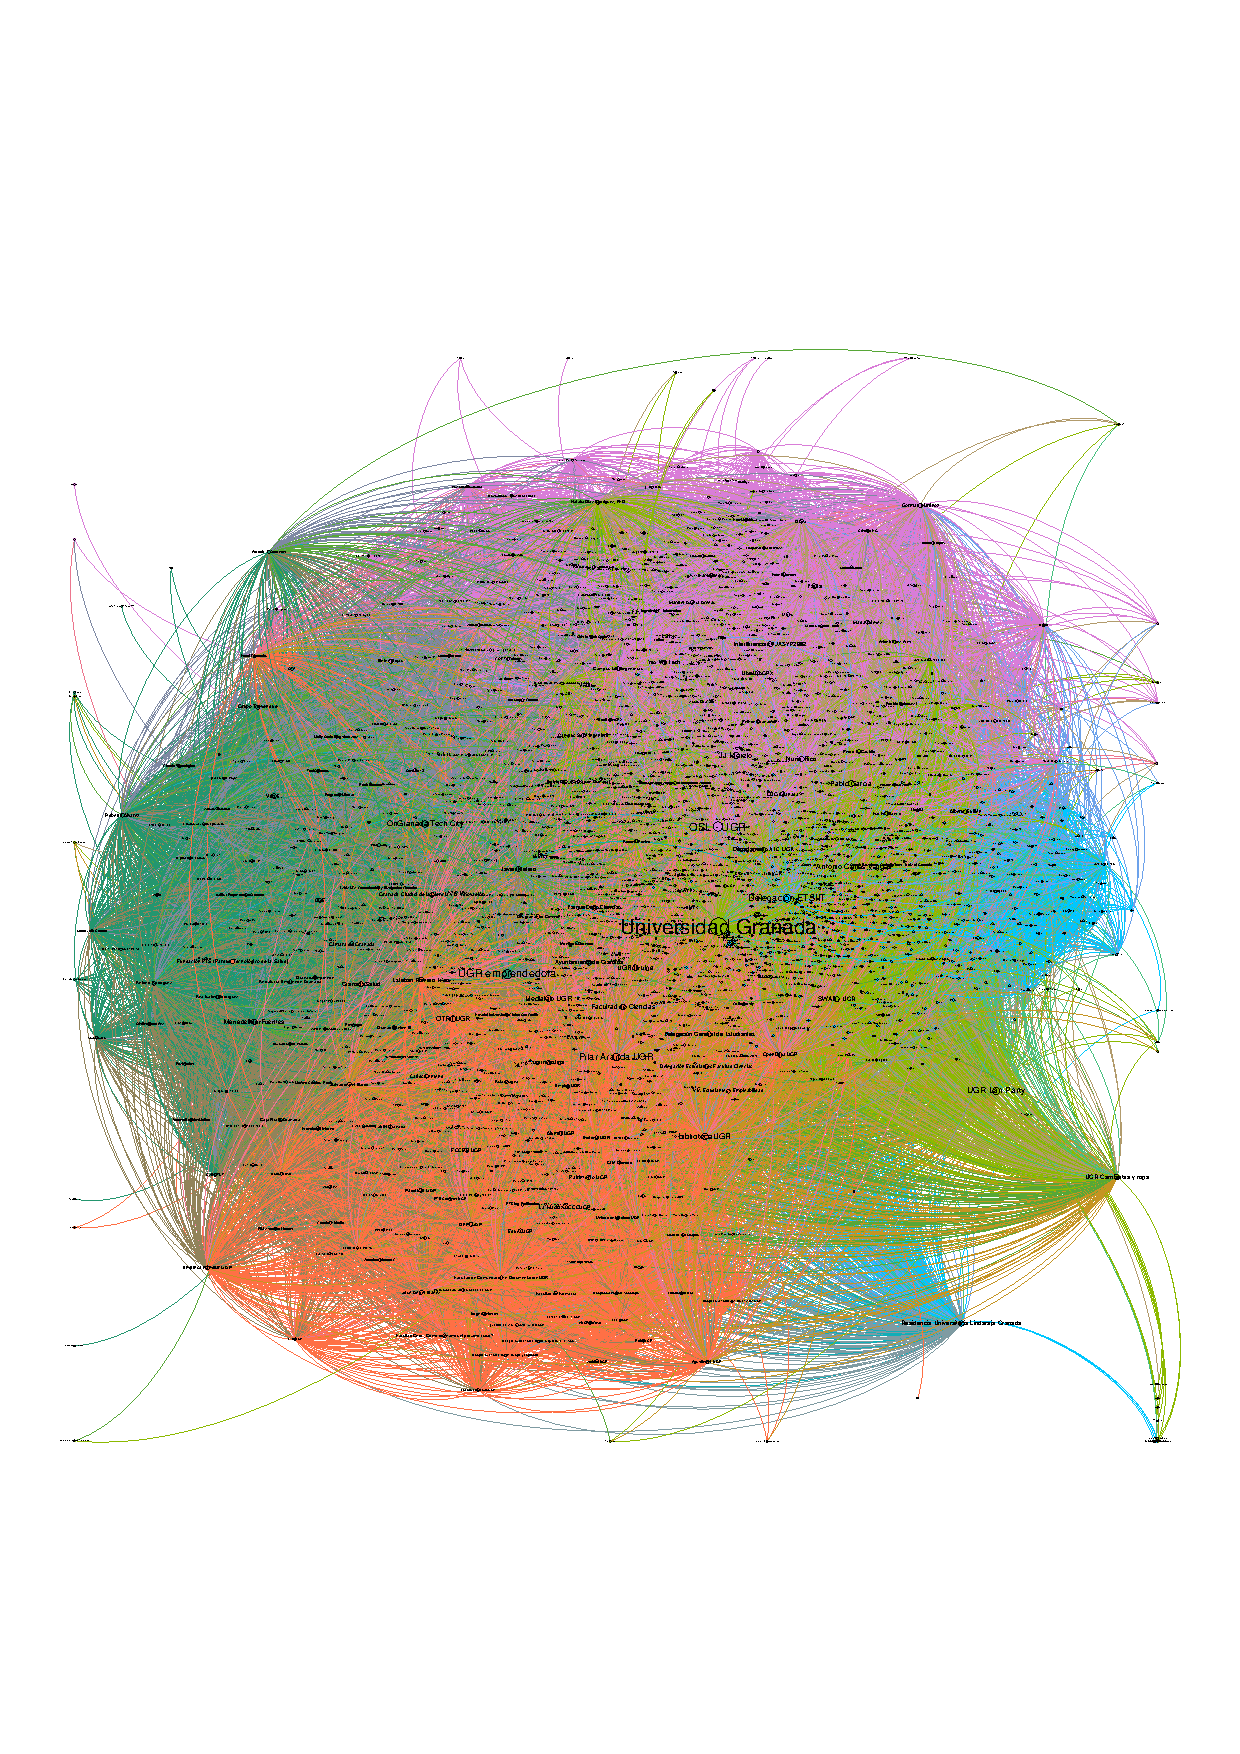
\includepdf[frame=true, scale=0.9, offset=75 -50]{pdf_incrustados/comunidades_lovaina_5.pdf}
	\caption{Red completa de seguidores de la cuenta ETSIIT, coloreada según comunidad y el tamaño de los nodos en función del grado.}
\end{figure}
\vspace{18cm}
En este caso podemos ver una división clara entre las comunidades de forma visual, aunque es cierto que, como era de esperar al analizar los actores principales, en las zonas de los nodos de la Universidad de Granada, la OSL, UGR Emprendedora y la Delegación de estudiantes de la ETSIIT, nodos importantes en la red que conectan muchas zonas, las comunidades se solapan. Por este motivo vamos a mostrarlas por separado y analizarlas una a una.
\newpage


\newpage
\begin{figure}[H]
	\centering
	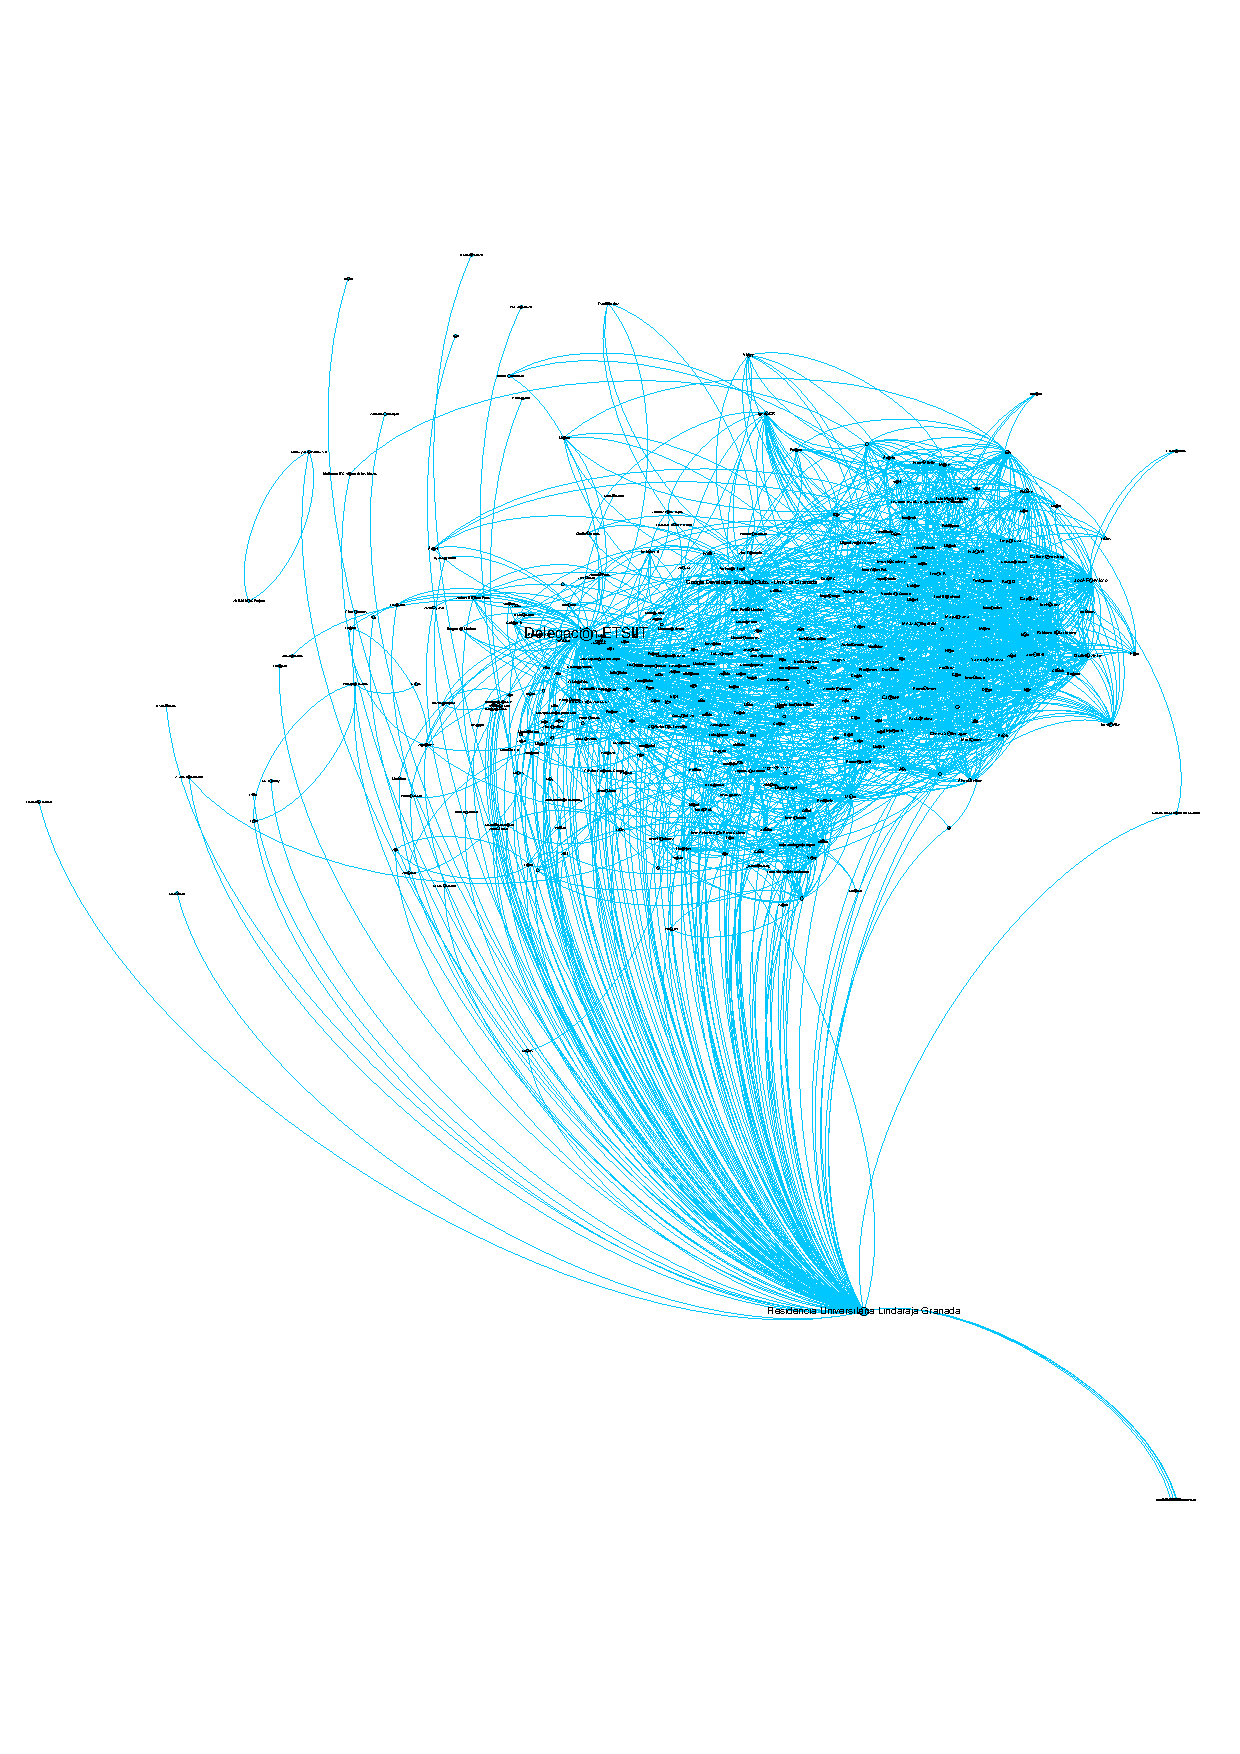
\includepdf[frame=true, scale=0.9, offset=75 -50]{pdf_incrustados/comunidades_lovaina_5_n0.pdf}
	\caption{Comunidad 0 de la red de seguidores de la cuenta ETSIIT, coloreada según comunidad y el tamaño de los nodos en función del grado.}
\end{figure}
\vspace{18cm}
En esta comunidad podemos observar como claramente se trata principalmente de una comunidad de estudiantes. Podemos encontrar la cuenta de la Delegación de estudiantes de la ETSIIT, la asociación de estudiantes Developer Student Clubs, así como otras cuentas personales, como mi propia cuenta o cuenta de conocidos de la ETSIIT, por lo que teniendo esa información experta podemos ver que esta comunidad cuadra claramente con estudiantes.
\newpage

\newpage
\begin{figure}[H]
	\centering
	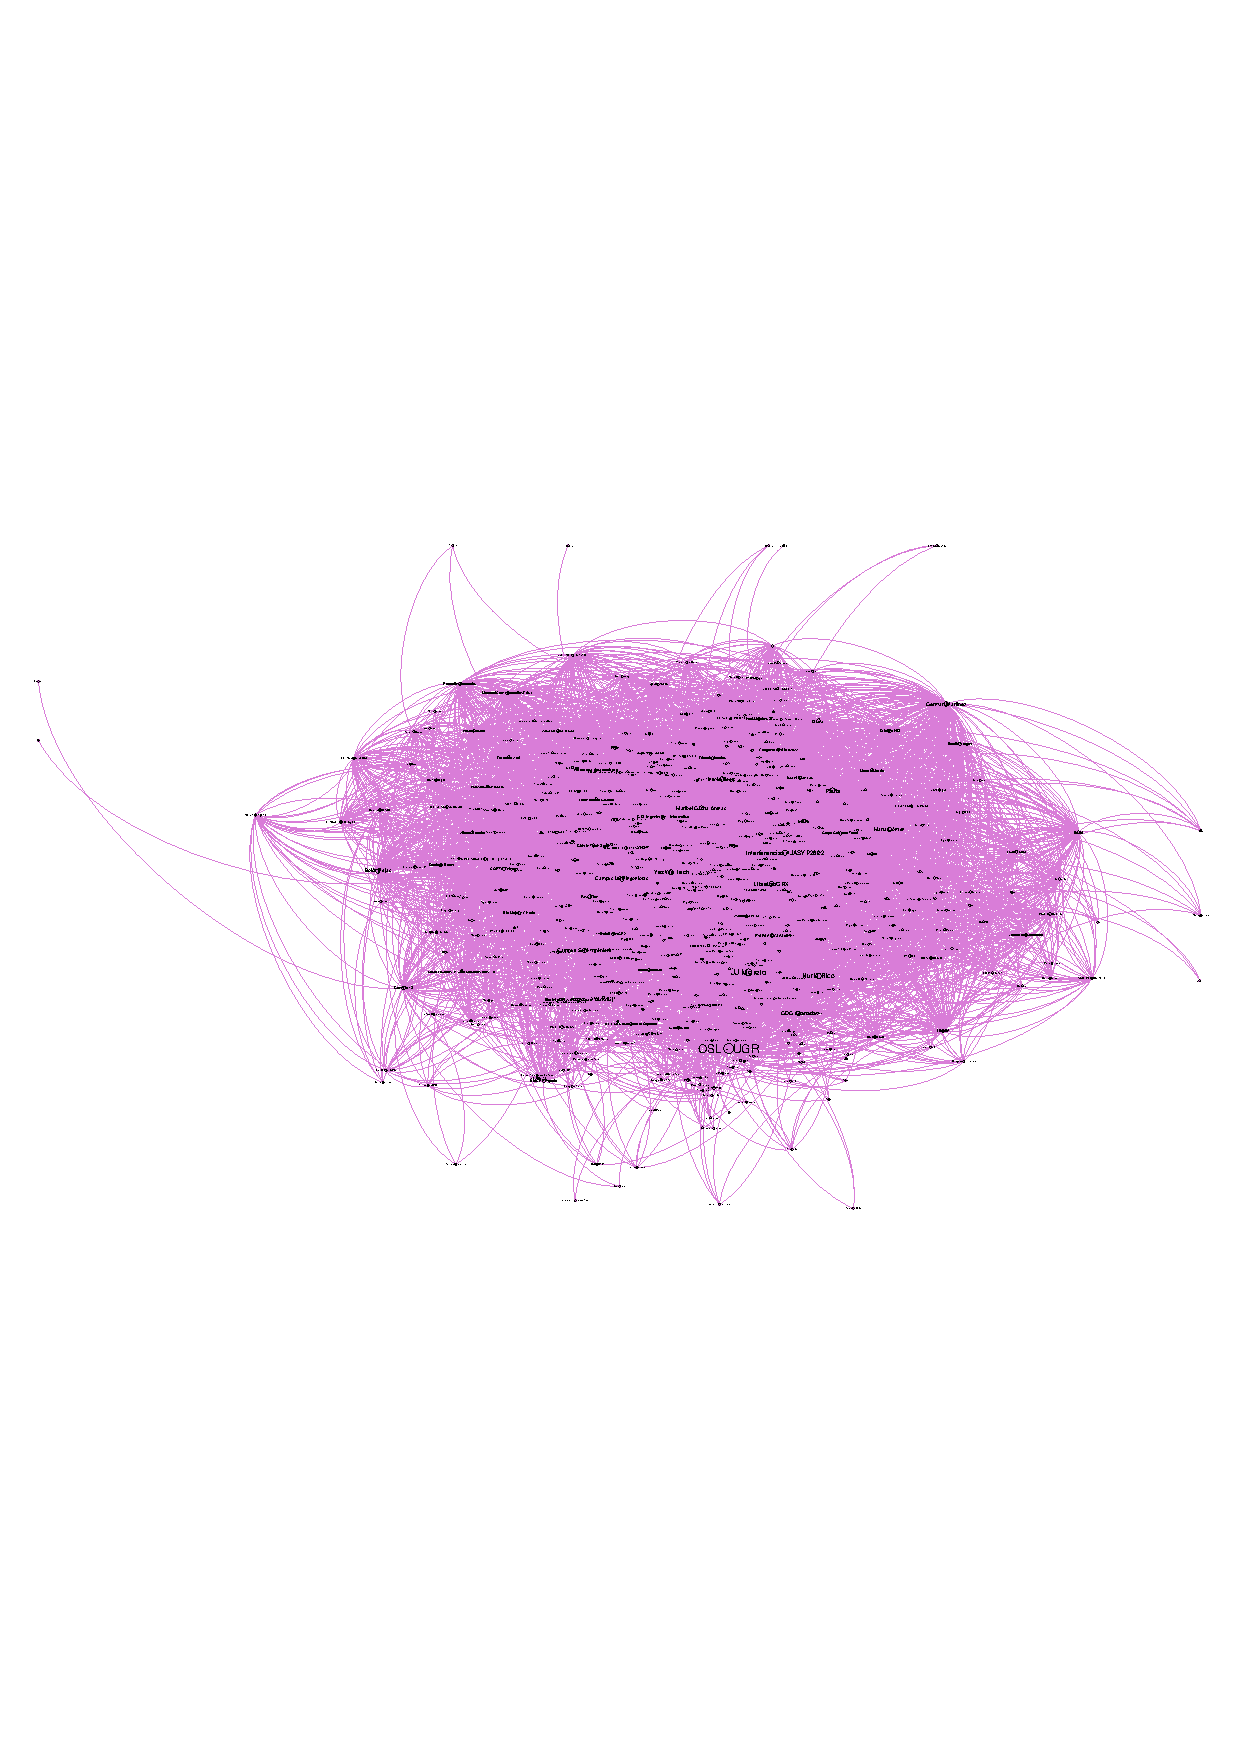
\includepdf[frame=true, scale=0.9, offset=75 -50]{pdf_incrustados/comunidades_lovaina_5_n1.pdf}
	\caption{Comunidad 1 de la red de seguidores de la cuenta ETSIIT, coloreada según comunidad y el tamaño de los nodos en función del grado.}
\end{figure}
\vspace{18cm}
Esta comunidad vemos como se trata de asociaciones relacionadas con la informática, como podemos ver con la OSL, LibreLabGRX, Interferencias, Yes We Tech, Campus UGRingenieras, entre otras asociaciones. Además, también podemos ver personas que forman parten o apoyan estas asociaciones, como JJ Merelo, Nuria Rico, Maribel García Arenas, entre otras cuentas.
\newpage


\newpage
\begin{figure}[H]
	\centering
	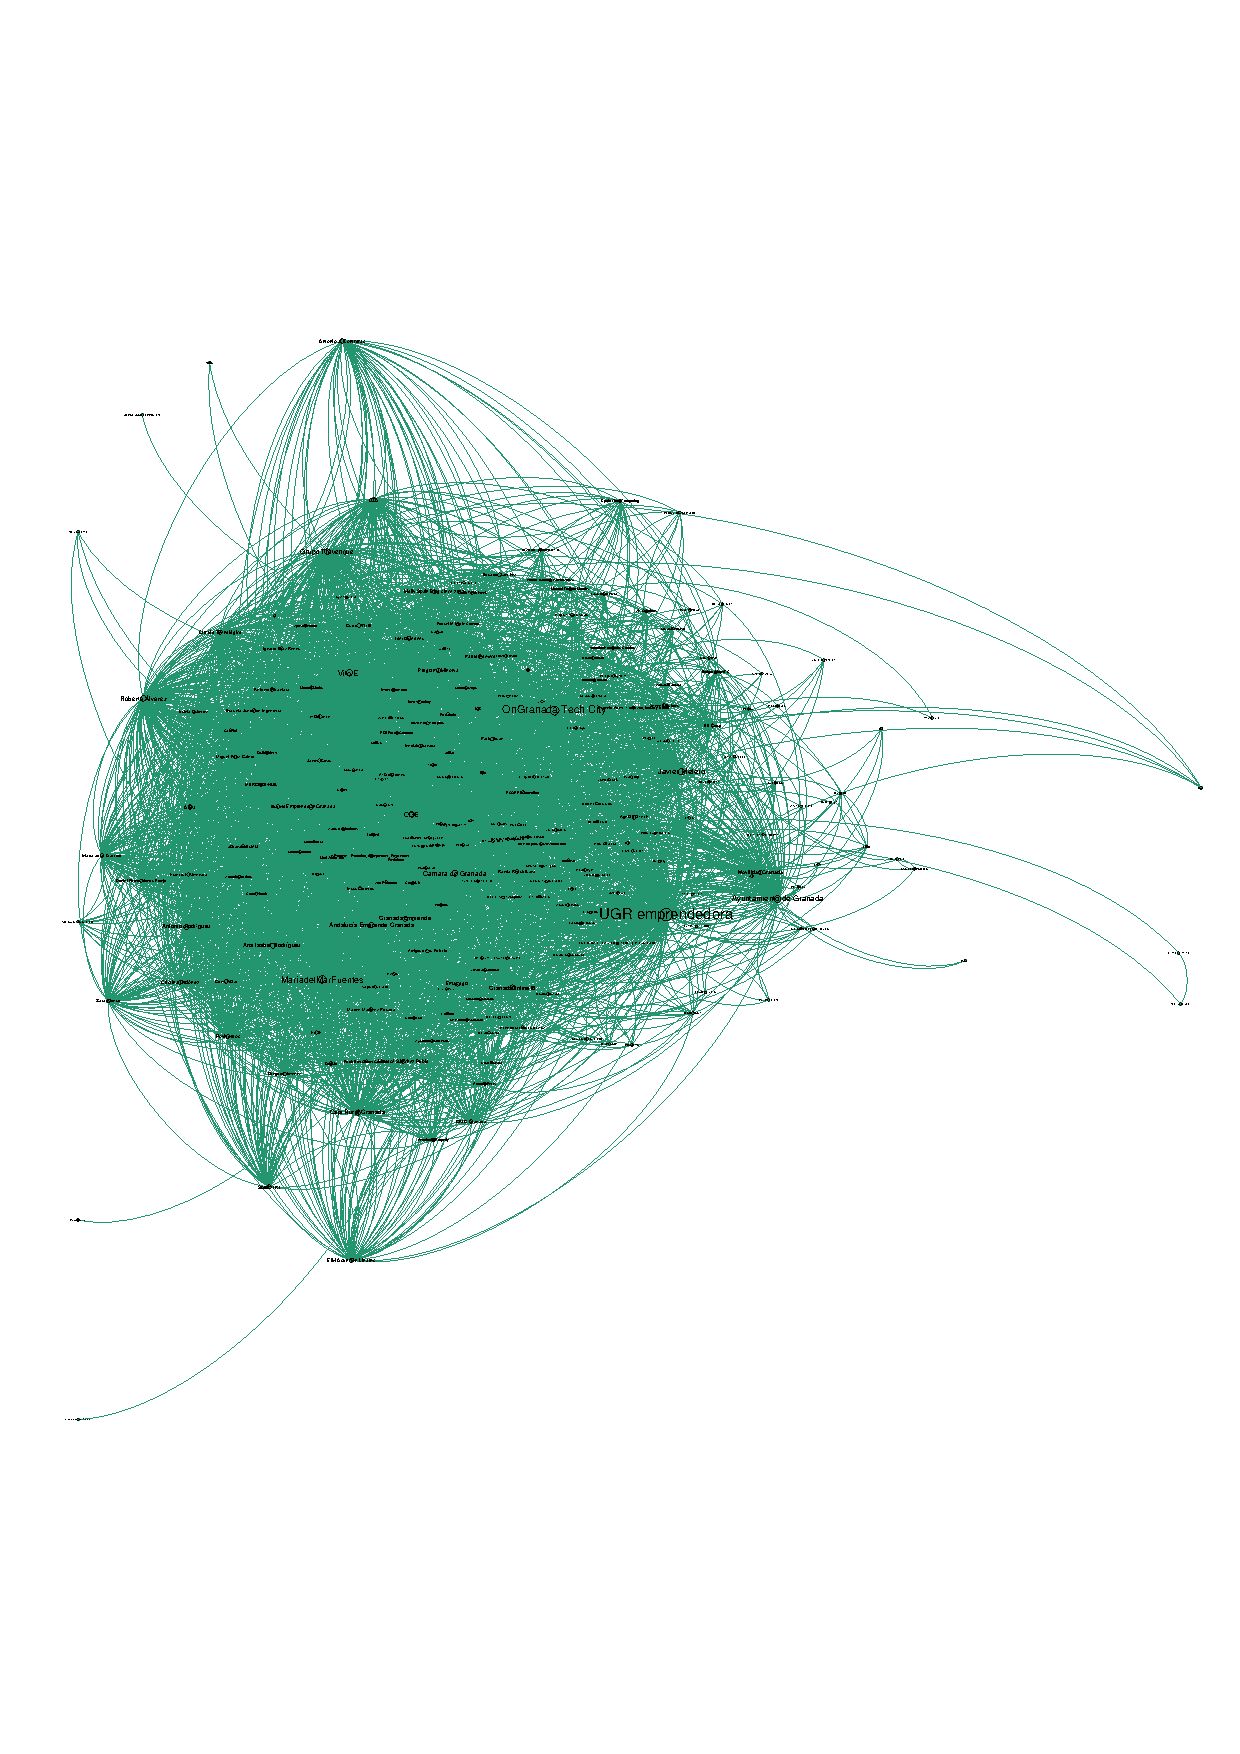
\includepdf[frame=true, scale=0.9, offset=75 -50]{pdf_incrustados/comunidades_lovaina_5_n2.pdf}
	\caption{Comunidad 2 de la red de seguidores de la cuenta ETSIIT, coloreada según comunidad y el tamaño de los nodos en función del grado.}
\end{figure}
\vspace{18cm}
Para esta comunidad se ve claramente que se tratan de cuentas asociadas a un sector más empresarial y de emprendimiento, como vemos están las cuentas de UGR Emprendedora, la Cámara de Comercio de Granada, OnGranada Tech City, incluso podemos ver cuentas de empresas como Caja Rural, Grupo Trevenque, entre otras.
\newpage


\newpage
\begin{figure}[H]
	\centering
	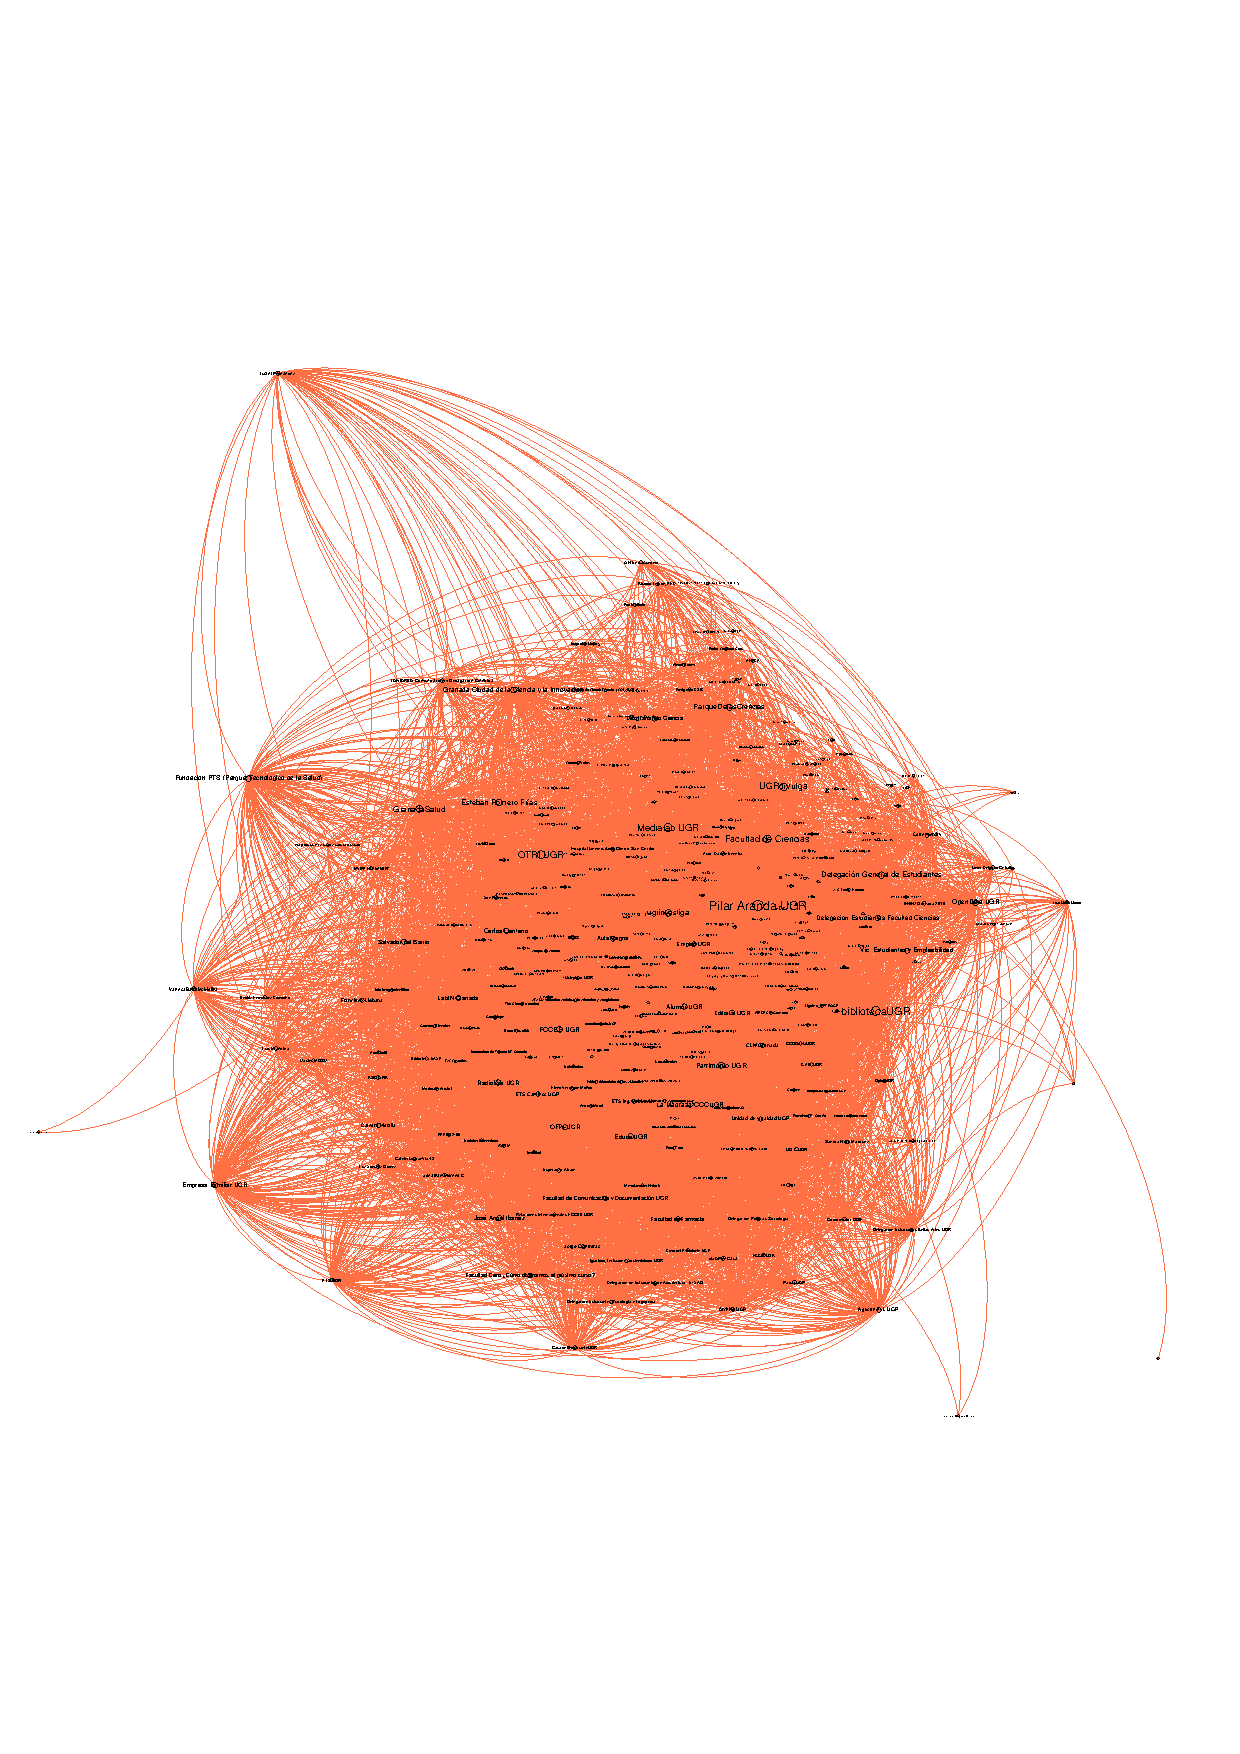
\includepdf[frame=true, scale=0.9, offset=75 -50]{pdf_incrustados/comunidades_lovaina_5_n3.pdf}
	\caption{Comunidad 3 de la red de seguidores de la cuenta ETSIIT, coloreada según comunidad y el tamaño de los nodos en función del grado.}
\end{figure}
\vspace{18cm}
Esta comunidad está formada principalmente por seguidores de la ETSIIT que forman parte de la UGR, como puede ser las cuentas de otras facultades de la UGR, servicios como bibliotecaUGR, los distintos vicerrectorados, entre otras cuentas de la UGR.
\newpage


\newpage
\begin{figure}[H]
	\centering
	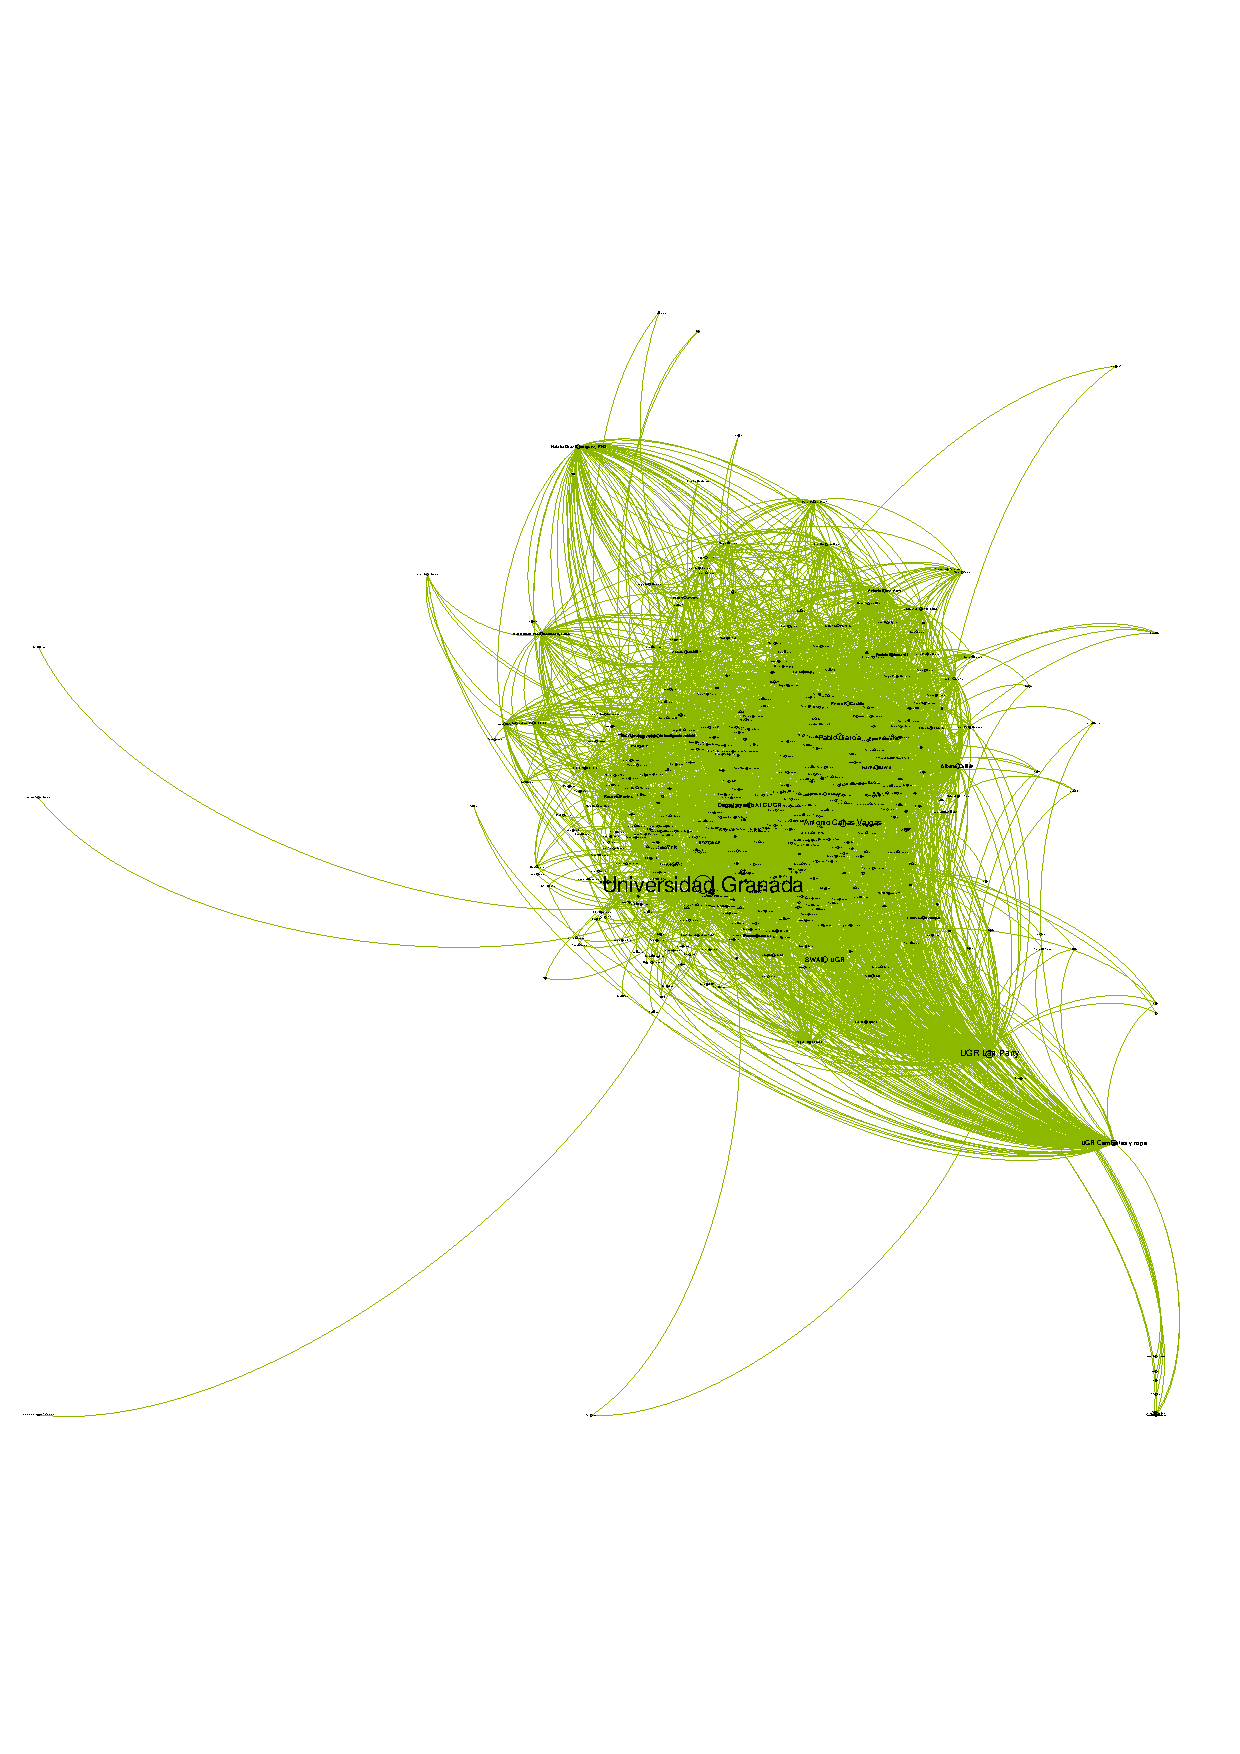
\includepdf[frame=true, scale=0.9, offset=75 -50]{pdf_incrustados/comunidades_lovaina_5_n4.pdf}
	\caption{Comunidad 4 de la red de seguidores de la cuenta ETSIIT, coloreada según comunidad y el tamaño de los nodos en función del grado.}
\end{figure}
\vspace{18cm}
Por último, esta comunidad vemos cuentas de profesores específicos de la UGR. Podemos encontrar la cuenta de Antonio Cañas, Pablo García, Alberto Guillén, Pedro A. Castillo, Francisco Herrera, la cuenta del departamento de ATC, etc.
\newpage

Como podemos ver en todas estas comunidades, todas tienen sentido y con podemos darles una explicación. Puede ser que el resultado tan bajo en modularidad se deba a que muchos de los nodos comparten distintas comunidades, como por ejemplo en la comunidad 1 y 4, muchos profesores de la ETSIIT también forman parte de las distintas asociaciones, pudiendo ser parte de ambos grupos. Sin embargo, gracias a este método y los métodos de visualización de ForceAtlas 2 vemos como podemos realizar una distinción bastante fácil y sacar conclusiones claras de estas comunidades, aunque hay que tener en cuenta estos detalles.


Si seguimos con una resolución más alta, vemos como se generan muy pocas comunidades, por lo que la información que aportan no es relevante:

% Please add the following required packages to your document preamble:
% \usepackage{graphicx}
\begin{table}[H]
\centering
\resizebox{\textwidth}{!}{%
\begin{tabular}{|r|r|r|r|r|}
\hline
\multicolumn{1}{|c|}{\textbf{Número de comunidad}} & \multicolumn{1}{c|}{\textbf{Número de nodos}} & \multicolumn{1}{c|}{\textbf{Porcentaje de nodos}} & \multicolumn{1}{c|}{\textbf{Número de enlaces}} & \multicolumn{1}{c|}{\textbf{Porcentaje de enlaces}} \\ \hline
\textit{Comunidad 0}                               & \textit{3}                                    & \textit{0,16}                                     & \textit{6}                                      & \textit{0,01}                                       \\ \hline
\textit{Comunidad 1}                               & \textit{860}                                  & \textit{46,44}                                    & \textit{20307}                                  & \textit{42,9}                                       \\ \hline
\textit{Comunidad 2}                               & \textit{989}                                  & \textit{53,4}                                     & \textit{16067}                                  & \textit{33,94}                                      \\ \hline
\end{tabular}%
}
\caption{Tres comunidades obtenidas para un valor de resolución de $1.5$.}
\end{table}

Además podemos ver que realmente son dos comunidades, ya que una de ellas tan solo cuenta con tres nodos y seis enlaces del total de la red.

Y si seguimos aumentando este valor, simplemente asignará una única comunidad con toda la red:

% Please add the following required packages to your document preamble:
% \usepackage{graphicx}
\begin{table}[H]
\centering
\resizebox{\textwidth}{!}{%
\begin{tabular}{|c|c|c|c|c|}
\hline
\textbf{Número de comunidad}               & \textbf{Número de nodos}           & \textbf{Porcentaje de nodos}      & \textbf{Número de enlaces}          & \textbf{Porcentaje de enlaces}    \\ \hline
\multicolumn{1}{|r|}{\textit{Comunidad 0}} & \multicolumn{1}{r|}{\textit{1852}} & \multicolumn{1}{r|}{\textit{100}} & \multicolumn{1}{r|}{\textit{47334}} & \multicolumn{1}{r|}{\textit{100}} \\ \hline
\end{tabular}%
}
\caption{Comunidad obtenida para un valor de resolución de $2.5$.}
\end{table}

\newpage

\subsection{Método de Leiden}

Tras utilizar el método de Leiden se han obtenido los siguientes resultados:

\begin{table}[H]
\centering
\begin{tabular}{|r|r|r|}
\hline
\multicolumn{1}{|c|}{\textbf{Resolución}} & \multicolumn{1}{c|}{\textbf{Calidad}} & \multicolumn{1}{c|}{\textbf{Número de comunidades}} \\ \hline
\textit{0,25}                             & \textit{0,75}                         & \textit{1}                                          \\ \hline
\textit{0,5}                              & \textit{0,5195}                       & \textit{2}                                          \\ \hline
\textit{1.0}                              & \textit{0,3099}                       & \textit{5}                                          \\ \hline
\textit{1,5}                              & \textit{0,2174}                       & \textit{12}                                         \\ \hline
\textit{2,5}                              & \textit{0,1357}                       & \textit{42}                                         \\ \hline
\end{tabular}
\end{table}

Como podemos ver, son resultados similares a los obtenidos con el método de Lovaina, sin embargo el primer detalle que puede llamar la atención es que el valor de la resolución funciona a la inversa que en el método de Leiden, es decir, a valores mayores de 1, el número de comunidades obtenidas aumenta, y no disminuye. Esto se debe a detalles de la implementación del plugin de Gephi.

Con respecto a las comunidades obtenidas, son muy similares a las obtenidas por Lovaina, con la diferencia de algunos nodos que se mueven a comunidades parecidas (como comenté en el apartado anterior al analizar las cinco comunidades obtenidas con resolución 1). Por este motivo, para no volver a repetir y extender esta memoria con las mismas conclusiones obtenidas en el apartado anterior, simplemente se va a visualizar las cinco particiones obtenidas con resolución 1:

\newpage
\begin{figure}[H]
	\centering
	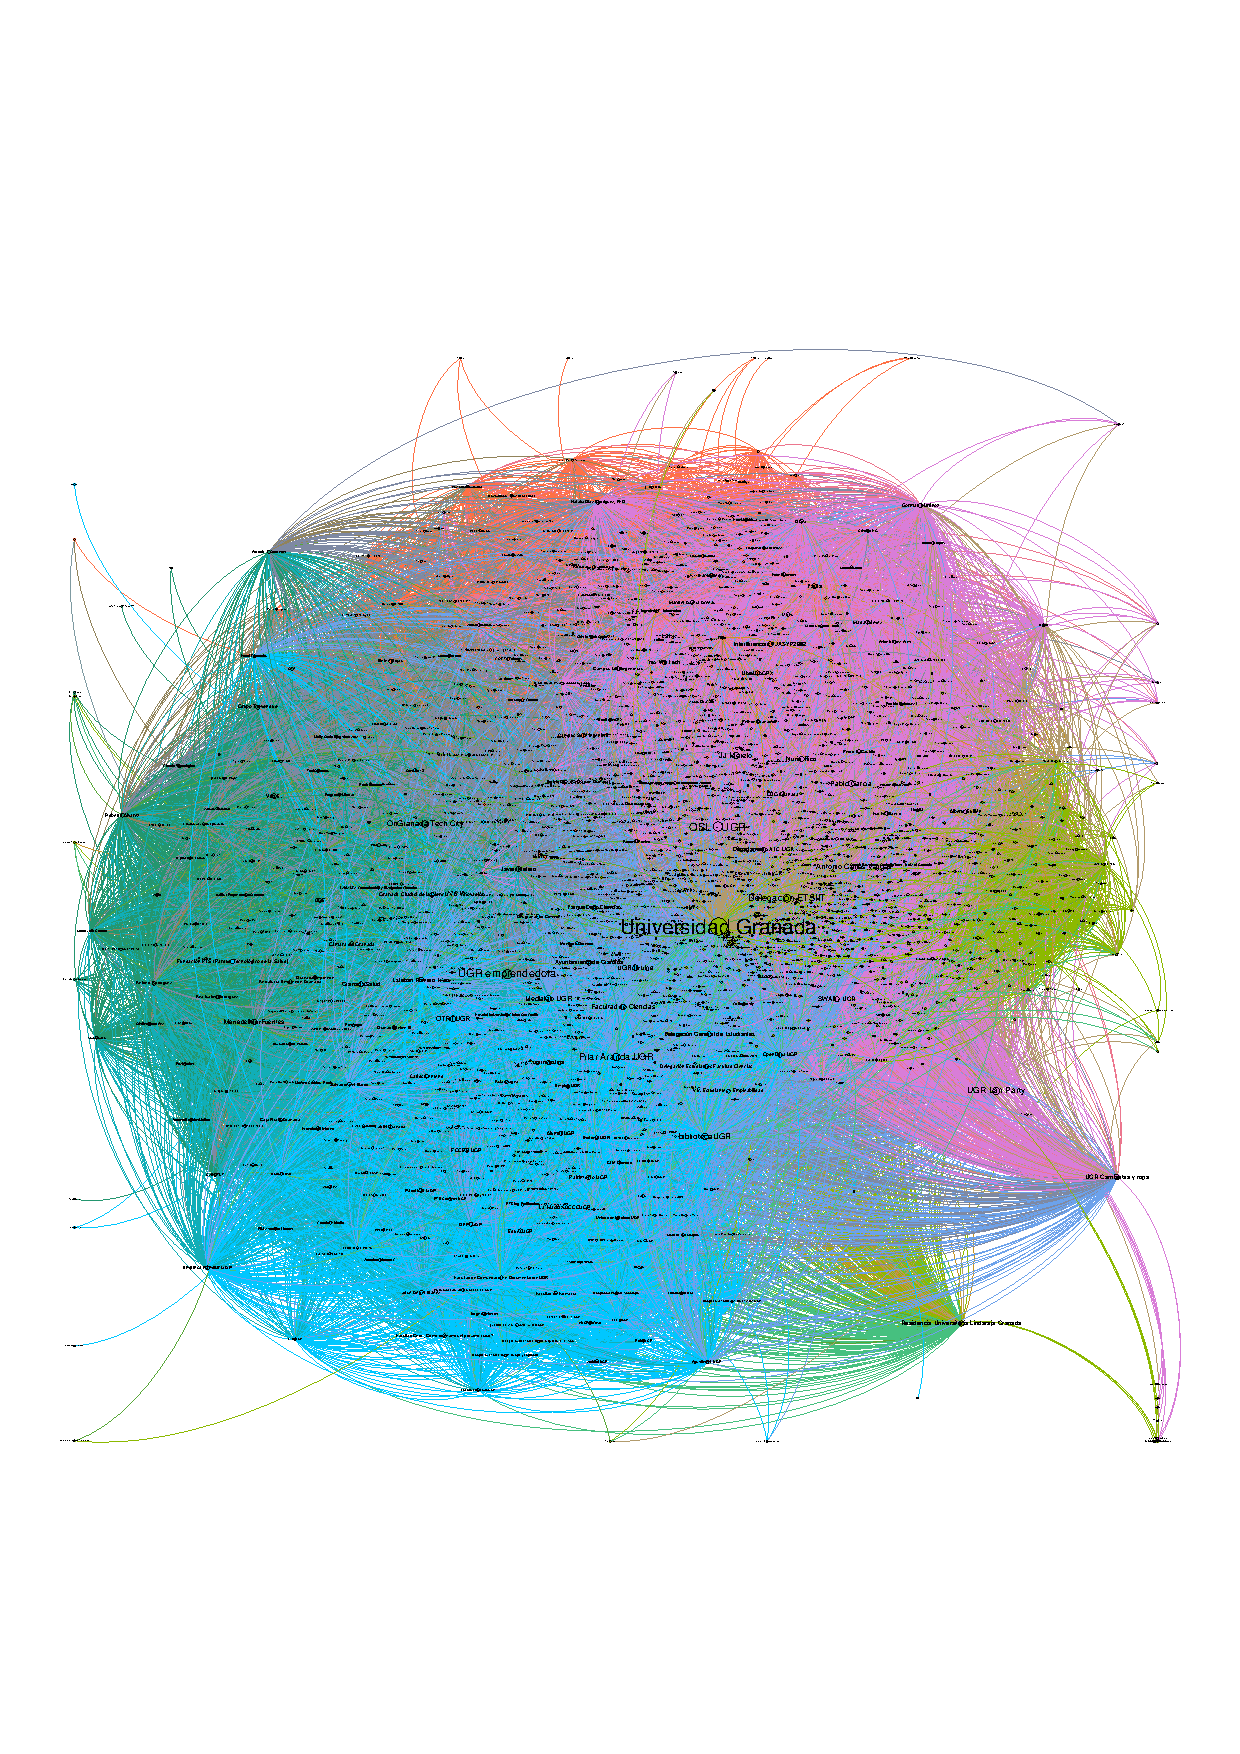
\includepdf[frame=true, scale=0.9, offset=75 -50]{pdf_incrustados/comunidades_leiden_5.pdf}
	\caption{Red completa de seguidores de la cuenta ETSIIT, coloreada según comunidad obtenida con el método de Leiden y el tamaño de los nodos en función del grado.}
\end{figure}
\vspace{18cm}
Vemos como en este caso el método de Leiden se ha comportado mejor al separar la comunidad de profesores y asociaciones de informática (comunidades 1 y 4 usando el método de Lovaina), separando mejor las cuentas personales de profesores de la ETSIIT con las cuentas de las asociaciones, en lugar de a los profesores involucrados en estas asociaciones unirlas a la comunidad de asociaciones.
\newpage

Como vemos, esta diferencia al asignar nodos a las comunidades puede ser o no relevante para extraer información de la red, dependiendo del enfoque que utilicemos podemos decir que ambas asignaciones son correctas.
